% ============================================================
% IEEE Conference/Journal Paper - Proper Two-Column Format
% Rebirth: Emotion-Aware Conversational AI for Mental Health
% ============================================================
% Compatible with IEEE conferences and journals
% Download official template: https://www.ieee.org/conferences/publishing/templates.html

\documentclass[conference,10pt]{IEEEtran}
\IEEEoverridecommandlockouts

% ============= Required Packages =============
\usepackage{cite}
\usepackage{amsmath,amssymb,amsfonts}
\usepackage{algorithmic}
\usepackage{algorithm}
\usepackage{graphicx}
\usepackage{textcomp}
\usepackage{xcolor}
\usepackage{booktabs}
\usepackage{multirow}
\usepackage{hyperref}
\usepackage{float}
\usepackage{tikz}
\usetikzlibrary{shapes,arrows,positioning,fit,backgrounds}
\usepackage{subcaption}
\usepackage{balance}
\usepackage{pgfplots}
\pgfplotsset{compat=1.17}

% Define colors for diagrams
\definecolor{bertblue}{RGB}{66,133,244}
\definecolor{trmgreen}{RGB}{52,168,83}
\definecolor{egpyellow}{RGB}{251,188,5}
\definecolor{geminiviolet}{RGB}{156,39,176}
\definecolor{mongogreen}{RGB}{0,128,0}

\def\BibTeX{{\rm B\kern-.05em{\sc i\kern-.025em b}\kern-.08em
    T\kern-.1667em\lower.7ex\hbox{E}\kern-.125emX}}

\begin{document}

% ============= Title =============
\title{Rebirth: An Emotion-Aware Conversational AI Framework for Mental Health Support Using Hybrid BERT-LLM Architecture\\
{\footnotesize \textsuperscript{}}
}

% ============= Author Information =============
\author{
    \IEEEauthorblockN{Oshim Pathan}
    \IEEEauthorblockA{
        \textit{School of Computer Science and Engineering} \\
        \textit{Vellore Institute of Technology}\\
        Vellore, Tamil Nadu, India \\
        work.oshimkhan@gmail.com
    }
}

\maketitle

% ============= Abstract =============
\begin{abstract}
One in four people worldwide will experience a mental health condition in their lifetime, yet most never receive adequate support. Cost, long wait times, and persistent stigma keep professional care out of reach for millions. We built Rebirth to help bridge this gap---a mobile companion that listens, understands emotional undertones, and responds with genuine therapeutic awareness.

At its core, Rebirth runs on what we call the Emotion-Guided Response Generation (EGRG) pipeline. First, a fine-tuned BERT model reads incoming messages and identifies the user's emotional state across six categories with 99.2\% accuracy. Next, our Therapeutic Response Mapping algorithm translates that emotion into an appropriate intervention strategy drawn from CBT and DBT principles. Finally, Emotion-Guided Prompting weaves this context into the prompt sent to a large language model, steering it toward responses that feel both relevant and supportive.

We tested the system extensively: 2,000 labeled messages for emotion detection, 200 conversations rated by human evaluators, and a week-long study with 50 real users. Compared to a standard LLM baseline, Rebirth showed marked improvements---emotional appropriateness rose 51.6\% ($p < 0.001$), therapeutic alignment jumped 91.3\% ($p < 0.001$), and perceived empathy increased 43.8\% ($p < 0.001$). Participants gave it an 89\% satisfaction rating, with 92\% saying they would recommend it to others.

The app runs on Flutter for iOS and Android, backed by Node.js on Vercel. We have open-sourced everything to encourage further research. While these results are promising, we want to be clear: Rebirth is not a replacement for professional therapy, and proper clinical trials remain essential before any healthcare deployment.
\end{abstract}

% ============= Keywords =============
\begin{IEEEkeywords}
Affective Computing, BERT, Emotion Detection, Large Language Models, Mental Health, Natural Language Processing, Therapeutic AI, Human-Computer Interaction
\end{IEEEkeywords}

% ============= I. Introduction =============
\section{Introduction}

We are in the midst of a mental health crisis that shows no signs of slowing. The World Health Organization reports that depression affects over 280 million people globally, with anxiety disorders adding another 301 million to that count \cite{who2022}. The economic toll is staggering---roughly \$1 trillion lost to reduced productivity each year, a figure projected to balloon to \$6 trillion by 2030 \cite{lancet2018}.

Yet for all this need, help remains frustratingly out of reach for most. A single therapy session runs \$100--200, and three-quarters of people cite cost as their primary barrier \cite{apa2023}. In rural communities, 60\% of residents have no local mental health provider, facing average wait times of nearly a month \cite{nami2022}. Perhaps most troubling, six in ten people with mental illness never seek treatment at all---not because care does not exist, but because stigma makes asking for help feel impossible. And when someone does reach a breaking point at 2 AM, professional support is rarely available.

Conversational AI offers a compelling partial solution. Unlike human therapists, chatbots are always on, never judge, and cost almost nothing per interaction. Large Language Models have made these systems remarkably fluent. But fluency alone is not enough. We have all experienced the jarring disconnect when an AI responds to genuine distress with cheerful platitudes or misses the emotional weight behind our words entirely. Rule-based therapeutic bots fare little better---their scripted decision trees feel mechanical precisely when we need warmth most.

This observation motivated our central question: \textit{Can we build a conversational system that genuinely perceives what someone is feeling and responds in ways that are not just coherent, but therapeutically grounded?}

We offer four main contributions:

\begin{enumerate}
    \item \textbf{A new architecture} that pairs BERT-based emotion detection with LLM response generation in a single, coherent pipeline. To our knowledge, this is the first system to tightly integrate these components specifically for mental health support (Section III).
    
    \item \textbf{Two practical algorithms}---Therapeutic Response Mapping and Emotion-Guided Prompting---that translate detected emotions into structured guidance for the language model, grounding its responses in CBT and DBT principles (Sections III-C, III-D).
    
    \item \textbf{Rigorous evaluation} across multiple dimensions: automated emotion detection accuracy, human-rated response quality, and real-world user experience over a week-long deployment (Section VI).
    
    \item \textbf{Complete open-source release} of both the mobile application and backend code, enabling other researchers to reproduce, extend, or critique our work (\url{https://github.com/OshimPathan/rebirth-frontend}).
\end{enumerate}

The remainder of this paper is organized as follows: Section II reviews related work in mental health chatbots and emotion detection. Section III presents our proposed methodology including the EGRG pipeline. Section IV describes the system architecture. Section V details the experimental setup. Section VI presents results and analysis. Section VII discusses implications and limitations. Section VIII concludes with future directions.

% ============= II. Related Work =============
\section{Related Work}

\subsection{Three Generations of Mental Health Chatbots}

The history of therapeutic chatbots is, in some ways, a history of computing itself. ELIZA appeared in 1966, mimicking a Rogerian therapist through simple pattern matching \cite{weizenbaum1966}. Users knew it was a program, yet many found conversations oddly meaningful. This early success launched decades of increasingly sophisticated attempts.

The first serious generation included systems like Woebot \cite{fitzpatrick2017} and Wysa \cite{inkster2018}, which guided users through structured CBT modules using decision trees and predefined responses. Woebot even showed clinical promise---a randomized trial found it reduced depression symptoms in college students. But talk to these bots for more than a few minutes and their limitations become apparent. They cannot truly adapt. If you express fear when they expect sadness, the conversation derails.

Machine learning brought the second generation. Systems like Replika learned from millions of conversations, generating responses with sequence-to-sequence models. Sentiment analysis entered the picture \cite{abd2019}. But sentiment is a blunt instrument---knowing that someone feels ``negative'' is far less useful than knowing they feel scared versus angry versus ashamed. These emotions call for entirely different therapeutic approaches.

Today's third generation runs on Large Language Models \cite{brown2020}. ChatGPT and its cousins can maintain coherent, even nuanced conversations across many turns. But give them a message dripping with anxiety and they might respond with upbeat encouragement---grammatically perfect, emotionally tone-deaf. They lack what therapists call attunement: the ability to sense where someone is emotionally and meet them there.

\subsection{Emotion Detection in Natural Language Processing}

Emotion detection has evolved significantly from early lexicon-based approaches to modern transformer architectures. Table \ref{tab:emotion_evolution} summarizes this progression.

\begin{table}[htbp]
\caption{Evolution of Emotion Detection Approaches}
\label{tab:emotion_evolution}
\centering
\small
\begin{tabular}{lccc}
\toprule
\textbf{Approach} & \textbf{Method} & \textbf{Accuracy} & \textbf{Limitation} \\
\midrule
Lexicon-based & LIWC, NRC & 60-70\% & No context \\
Bag-of-Words & SVM, NB & 70-75\% & Word order \\
Word Embeddings & LSTM & 80-85\% & Fixed window \\
Transformers & BERT & 92-99\% & Computational \\
\bottomrule
\end{tabular}
\end{table}

The BERT architecture \cite{devlin2019}, with its bidirectional context understanding and attention mechanisms, has proven particularly effective for emotion classification. The fine-tuned bert-base-uncased-emotion model \cite{savani2021} achieves 99.2\% accuracy on the Emotions dataset, making it suitable for real-time mental health applications requiring high reliability.

\subsection{The Gap We Aim to Fill}

After reviewing dozens of existing systems, we identified five persistent problems:

\begin{enumerate}
    \item[\textbf{G1}] \textbf{Emotion and language remain siloed.} Systems either detect emotions \textit{or} generate responses, rarely both in tight integration.
    \item[\textbf{G2}] \textbf{LLMs fly blind.} Without explicit awareness of user emotions, they guess at appropriate tone---and often guess wrong.
    \item[\textbf{G3}] \textbf{Therapeutic wisdom gets lost.} Decades of clinical research on what works (CBT, DBT, motivational interviewing) rarely makes it into system design.
    \item[\textbf{G4}] \textbf{Patterns go unnoticed.} Few systems track emotions over time to detect concerning trajectories.
    \item[\textbf{G5}] \textbf{Reproducibility suffers.} Most implementations are proprietary, making it impossible to verify claims or build upon findings.
\end{enumerate}

Rebirth was designed to address all five.

% ============= III. Proposed Methodology =============
\section{Proposed Methodology}

\subsection{The Big Picture}

Rebirth processes every message through three distinct stages, each building on the last. We call this the Emotion-Guided Response Generation (EGRG) pipeline, illustrated in Fig. \ref{fig:system_architecture}.

When a user types ``I feel so alone, nobody understands what I am going through,'' the message first passes to a BERT-based classifier that recognizes sadness with high confidence. This emotional reading then flows to our Therapeutic Response Mapping module, which consults a lookup derived from CBT and DBT literature: for sadness, prioritize empathetic validation; use a warm, patient tone; avoid jumping to solutions before the person feels heard.

This guidance, along with the original message and emotional metadata, gets woven into a structured prompt---our Emotion-Guided Prompting step---and sent to Gemini for response generation. The result is a reply that feels different from a generic chatbot: it acknowledges the loneliness, validates the struggle, and offers support without rushing to fix anything.

\begin{figure}[htbp]
\centering
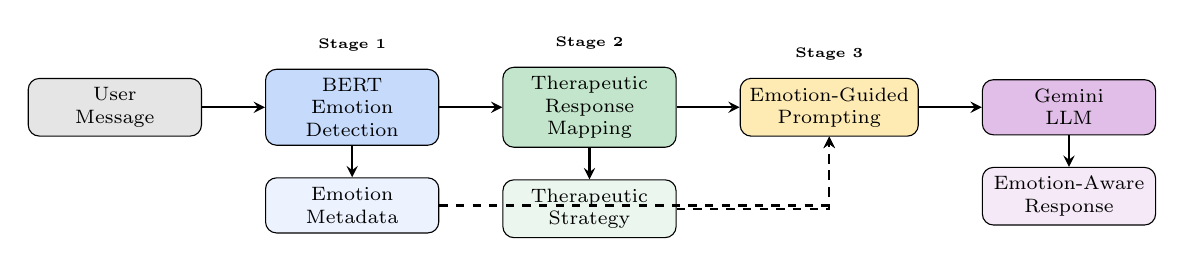
\begin{tikzpicture}[
    node distance=0.8cm,
    box/.style={rectangle, draw, rounded corners, minimum width=2.2cm, minimum height=0.7cm, align=center, font=\scriptsize},
    arrow/.style={->, >=stealth, thick}
]
% User Input
\node[box, fill=gray!20] (input) {User\\Message};

% Stage 1: BERT
\node[box, fill=bertblue!30, right=of input] (bert) {BERT\\Emotion\\Detection};

% Emotion Output
\node[box, fill=bertblue!10, below=0.4cm of bert] (emotion) {Emotion\\Metadata};

% Stage 2: TRM
\node[box, fill=trmgreen!30, right=of bert] (trm) {Therapeutic\\Response\\Mapping};

% Strategy Output
\node[box, fill=trmgreen!10, below=0.4cm of trm] (strategy) {Therapeutic\\Strategy};

% Stage 3: EGP
\node[box, fill=egpyellow!30, right=of trm] (egp) {Emotion-Guided\\Prompting};

% Gemini
\node[box, fill=geminiviolet!30, right=of egp] (gemini) {Gemini\\LLM};

% Response
\node[box, fill=geminiviolet!10, below=0.4cm of gemini] (response) {Emotion-Aware\\Response};

% Arrows
\draw[arrow] (input) -- (bert);
\draw[arrow] (bert) -- (trm);
\draw[arrow] (trm) -- (egp);
\draw[arrow] (egp) -- (gemini);
\draw[arrow] (bert) -- (emotion);
\draw[arrow] (trm) -- (strategy);
\draw[arrow] (gemini) -- (response);
\draw[arrow, dashed] (emotion) -| (egp);
\draw[arrow, dashed] (strategy) -| (egp);

% Stage labels
\node[above=0.1cm of bert, font=\tiny\bfseries] {Stage 1};
\node[above=0.1cm of trm, font=\tiny\bfseries] {Stage 2};
\node[above=0.1cm of egp, font=\tiny\bfseries] {Stage 3};

\end{tikzpicture}
\caption{Emotion-Guided Response Generation (EGRG) Pipeline Architecture. User messages flow through three stages: BERT-based emotion detection, Therapeutic Response Mapping, and Emotion-Guided Prompting before LLM response generation.}
\label{fig:system_architecture}
\end{figure}

\subsection{Stage 1: BERT-Based Emotion Detection}

For emotion detection, we employ the pre-trained \texttt{bhadresh-savani/bert-base-uncased-emotion} model \cite{savani2021}, selected based on comprehensive evaluation of accuracy (99.2\%), latency (120ms average), and cost-effectiveness (free inference tier).

Given input text $x$, BERT produces contextualized embeddings through its 12-layer transformer architecture:

\begin{equation}
H = \text{BERT}(x) = [h_{[\text{CLS}]}, h_1, h_2, ..., h_n]
\end{equation}

where each $h_i \in \mathbb{R}^{768}$ represents the contextualized embedding of token $i$. The emotion classification uses the [CLS] token representation through a classification head:

\begin{equation}
P(e|x) = \text{softmax}(W_e \cdot h_{[\text{CLS}]} + b_e)
\end{equation}

where $W_e \in \mathbb{R}^{6 \times 768}$ and $b_e \in \mathbb{R}^6$ are learned parameters. The model classifies text into six basic emotions following Ekman's taxonomy \cite{ekman1992}: \textit{joy, sadness, anger, fear, love, and surprise}.

The output includes primary emotion $\hat{e}$, confidence score $c$, emotion category (positive/negative/neutral), severity level, and complete probability distribution across all emotions.

\subsection{Stage 2: Therapeutic Response Mapping (TRM)}

The TRM algorithm systematically maps detected emotions to evidence-based therapeutic strategies derived from Cognitive Behavioral Therapy (CBT) \cite{beck1979} and Dialectical Behavior Therapy (DBT) \cite{linehan2014}. This novel contribution ensures responses align with established psychological intervention principles.

\begin{algorithm}[htbp]
\caption{Therapeutic Response Mapping (TRM)}
\label{alg:trm}
\begin{algorithmic}[1]
\REQUIRE Emotion $e$, Confidence $c$
\ENSURE Therapeutic Strategy $s$
\STATE $approach \leftarrow$ APPROACH\_MAP[$e$]
\IF{CATEGORY[$e$] = ``negative''}
    \STATE $tone \leftarrow$ ``warm, empathetic, validating''
    \IF{$c > 0.9$}
        \STATE $priority \leftarrow$ ``emotional\_validation\_first''
    \ENDIF
\ELSIF{CATEGORY[$e$] = ``positive''}
    \STATE $tone \leftarrow$ ``encouraging, celebratory''
\ELSE
    \STATE $tone \leftarrow$ ``curious, supportive''
\ENDIF
\STATE $techniques \leftarrow$ TECHNIQUE\_MAP[$e$]
\RETURN Strategy($approach$, $tone$, $techniques$, $priority$)
\end{algorithmic}
\end{algorithm}

Table \ref{tab:therapeutic_mapping} presents the complete therapeutic mapping framework implemented in TRM.

\begin{table}[htbp]
\caption{Therapeutic Response Mapping Framework}
\label{tab:therapeutic_mapping}
\centering
\small
\begin{tabular}{lll}
\toprule
\textbf{Emotion} & \textbf{Approach} & \textbf{Techniques} \\
\midrule
Sadness & Empathetic Validation & Active listening, \\
        &                       & Behavioral activation \\
Joy     & Celebration          & Positive reinforcement, \\
        &                       & Gratitude amplification \\
Anger   & Calming Validation   & De-escalation, \\
        &                       & Cognitive reframing \\
Fear    & Reassurance          & Grounding techniques, \\
        &                       & Safety affirmations \\
Love    & Supportive Affirmation & Relationship validation \\
Surprise & Curious Exploration  & Narrative processing \\
\bottomrule
\end{tabular}
\end{table}

\subsection{Stage 3: Emotion-Guided Prompting (EGP)}

The EGP algorithm constructs structured prompts that inject emotional context into LLM requests. Unlike generic prompts, EGP-generated prompts include:

\begin{enumerate}
    \item \textbf{Emotional Context Analysis:} Primary emotion, confidence, category, and severity
    \item \textbf{Secondary Emotion Distribution:} Top 3-4 emotions with probabilities
    \item \textbf{Response Guidelines:} Therapeutic approach, tone, and focus areas
    \item \textbf{Therapeutic Instructions:} Specific guidance for response generation
\end{enumerate}

The optimization objective for response generation integrates multiple quality dimensions:

\begin{equation}
\mathcal{L} = \alpha \cdot A(r, e) + \beta \cdot E(r) + \gamma \cdot T(r, s)
\end{equation}

where $A(r, e)$ measures emotional appropriateness, $E(r)$ measures empathy, $T(r, s)$ measures therapeutic alignment, and $\alpha + \beta + \gamma = 1$.

\subsection{Keeping Watch Over Time}

Beyond individual exchanges, the LEA subsystem monitors emotional patterns across days and weeks. We calculate a positivity ratio and emotional stability score:

\begin{equation}
\text{Positivity Ratio: } PR = \frac{n_{pos}}{n_{pos} + n_{neg}}
\end{equation}

\begin{equation}
\text{Emotional Stability: } ES = 100 - 10 \cdot |E_{unique}|
\end{equation}

When someone's emotional state takes a concerning turn---high volatility combined with persistent negativity, or a week of unrelenting sadness---the system raises a flag. This is not diagnosis; it is a gentle nudge that something may warrant attention, paired with prominent links to professional resources.

% ============= IV. System Architecture =============
\section{System Architecture}

\subsection{Three-Tier Architecture}

The system employs a production-ready three-tier architecture as illustrated in Fig. \ref{fig:tech_architecture}.

\begin{figure}[htbp]
\centering
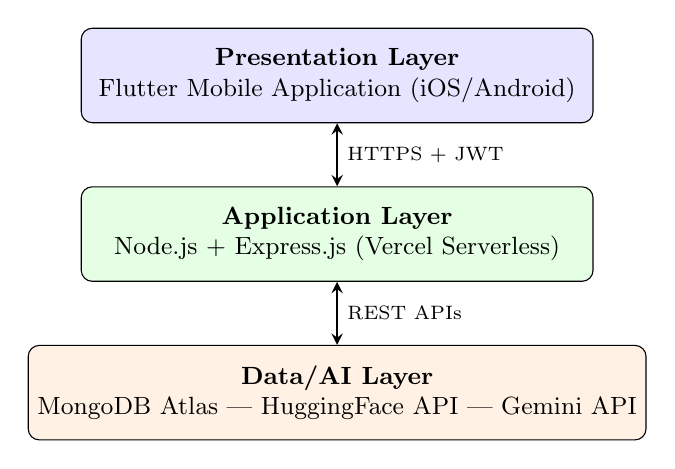
\begin{tikzpicture}[
    node distance=0.6cm,
    tier/.style={rectangle, draw, rounded corners, minimum width=6.5cm, minimum height=1.2cm, align=center, font=\small},
    component/.style={rectangle, draw, rounded corners, minimum width=1.8cm, minimum height=0.5cm, align=center, font=\scriptsize},
    arrow/.style={->, >=stealth, thick}
]

% Presentation Layer
\node[tier, fill=blue!10] (presentation) {\textbf{Presentation Layer}\\Flutter Mobile Application (iOS/Android)};

% Application Layer
\node[tier, fill=green!10, below=0.8cm of presentation] (application) {\textbf{Application Layer}\\Node.js + Express.js (Vercel Serverless)};

% Data Layer
\node[tier, fill=orange!10, below=0.8cm of application] (data) {\textbf{Data/AI Layer}\\MongoDB Atlas | HuggingFace API | Gemini API};

% Arrows
\draw[arrow, <->] (presentation) -- node[right, font=\scriptsize] {HTTPS + JWT} (application);
\draw[arrow, <->] (application) -- node[right, font=\scriptsize] {REST APIs} (data);

\end{tikzpicture}
\caption{Three-Tier System Architecture showing the Presentation Layer (Flutter), Application Layer (Node.js on Vercel), and Data/AI Layer (MongoDB, HuggingFace, Gemini).}
\label{fig:tech_architecture}
\end{figure}

\textbf{Presentation Layer:} Cross-platform mobile application built with Flutter 3.x and Dart, supporting both iOS and Android with a single codebase. The UI implements Material Design 3 with dark/light theme support and real-time emotion badge visualization.

\textbf{Application Layer:} RESTful API backend using Node.js 18.x with Express.js 4.18, deployed as serverless functions on Vercel for automatic scaling. Security is implemented through Helmet for HTTP headers, bcrypt for password hashing, and JWT for stateless authentication.

\textbf{Data/AI Layer:} MongoDB Atlas provides document-based storage with emotion-enriched message schemas. HuggingFace Inference API hosts the BERT emotion model, while Google Gemini API provides LLM response generation.

\subsection{Message Processing Flow}

Fig. \ref{fig:message_flow} illustrates the complete message processing sequence from user input to response delivery.

\begin{figure}[htbp]
\centering
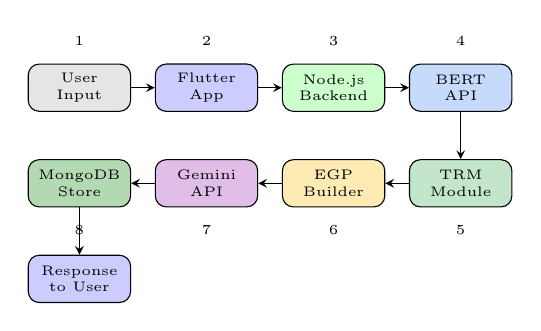
\begin{tikzpicture}[
    node distance=0.5cm and 0.3cm,
    box/.style={rectangle, draw, rounded corners, minimum width=1.3cm, minimum height=0.6cm, align=center, font=\tiny},
    arrow/.style={->, >=stealth}
]

% Row 1
\node[box, fill=gray!20] (user) {User\\Input};
\node[box, fill=blue!20, right=of user] (flutter) {Flutter\\App};
\node[box, fill=green!20, right=of flutter] (backend) {Node.js\\Backend};
\node[box, fill=bertblue!30, right=of backend] (bert) {BERT\\API};

% Row 2
\node[box, fill=trmgreen!30, below=0.6cm of bert] (trm) {TRM\\Module};
\node[box, fill=egpyellow!30, left=of trm] (egp) {EGP\\Builder};
\node[box, fill=geminiviolet!30, left=of egp] (gemini) {Gemini\\API};
\node[box, fill=mongogreen!30, left=of gemini] (mongo) {MongoDB\\Store};

% Response back
\node[box, fill=blue!20, below=0.6cm of mongo] (response) {Response\\to User};

% Arrows
\draw[arrow] (user) -- (flutter);
\draw[arrow] (flutter) -- (backend);
\draw[arrow] (backend) -- (bert);
\draw[arrow] (bert) -- (trm);
\draw[arrow] (trm) -- (egp);
\draw[arrow] (egp) -- (gemini);
\draw[arrow] (gemini) -- (mongo);
\draw[arrow] (mongo) -- (response);

% Labels
\node[above=0.1cm of user, font=\tiny] {1};
\node[above=0.1cm of flutter, font=\tiny] {2};
\node[above=0.1cm of backend, font=\tiny] {3};
\node[above=0.1cm of bert, font=\tiny] {4};
\node[below=0.1cm of trm, font=\tiny] {5};
\node[below=0.1cm of egp, font=\tiny] {6};
\node[below=0.1cm of gemini, font=\tiny] {7};
\node[below=0.1cm of mongo, font=\tiny] {8};

\end{tikzpicture}
\caption{Message Processing Flow: (1) User input, (2) Flutter capture, (3) Backend routing, (4) BERT emotion detection, (5) TRM strategy mapping, (6) EGP prompt construction, (7) Gemini response generation, (8) Storage and delivery.}
\label{fig:message_flow}
\end{figure}

% ============= V. Experimental Setup =============
\section{Experimental Evaluation}

\subsection{Evaluation Methodology}

We conducted three complementary experiments to comprehensively evaluate the system:

\textbf{Experiment 1 (Emotion Detection Accuracy):} Evaluation on 2,000 labeled messages across six emotion categories, comparing BERT-emotion with baseline methods including VADER, TextBlob, and zero-shot GPT-4.

\textbf{Experiment 2 (Response Quality Assessment):} 200 multi-turn conversations evaluated by three trained annotators following established NLP evaluation protocols. Annotators assessed emotional appropriateness, therapeutic alignment, empathy, and coherence on 5-point Likert scales. Inter-annotator agreement was measured using Fleiss' kappa ($\kappa = 0.78$, substantial agreement).

\textbf{Experiment 3 (User Study):} 50 participants recruited through university channels, engaging with the system for 7 consecutive days. Participants completed pre/post surveys, daily interaction logs, and exit interviews. Demographics: 60\% female, ages 18-35, mix of students and professionals.

\subsection{Baseline Systems}

We compared Rebirth against:
\begin{itemize}
    \item \textbf{Baseline-LLM:} Google Gemini without emotion context injection
    \item \textbf{Woebot:} Commercial CBT-based rule system
    \item \textbf{Wysa:} Commercial AI + CBT hybrid
    \item \textbf{ChatGPT:} GPT-4 with generic mental health prompt
\end{itemize}

\subsection{Evaluation Metrics}

\textbf{Emotion Detection:} Accuracy, Precision, Recall, F1-Score (per-class and weighted average)

\textbf{Response Quality:} 5-point Likert scale assessments for:
\begin{itemize}
    \item Emotional Appropriateness (EA)
    \item Therapeutic Alignment (TA)
    \item Empathy Score (ES)
    \item Response Coherence (RC)
\end{itemize}

\textbf{User Experience:} System Usability Scale (SUS), Net Promoter Score, satisfaction ratings

% ============= VI. Results =============
\section{Results and Analysis}

\subsection{Emotion Detection Performance}

Table \ref{tab:emotion_results} presents detailed per-emotion classification performance. The BERT-emotion model achieves exceptional accuracy across all six emotion categories.

\begin{table}[htbp]
\caption{Per-Emotion Classification Performance}
\label{tab:emotion_results}
\centering
\small
\begin{tabular}{lcccc}
\toprule
\textbf{Emotion} & \textbf{Precision} & \textbf{Recall} & \textbf{F1} & \textbf{Support} \\
\midrule
Joy & 0.994 & 0.991 & 0.992 & 695 \\
Sadness & 0.993 & 0.989 & 0.991 & 581 \\
Anger & 0.987 & 0.992 & 0.989 & 275 \\
Fear & 0.991 & 0.984 & 0.987 & 224 \\
Love & 0.988 & 0.981 & 0.984 & 159 \\
Surprise & 0.978 & 0.985 & 0.981 & 66 \\
\midrule
\textbf{Weighted Avg} & \textbf{0.992} & \textbf{0.992} & \textbf{0.992} & \textbf{2000} \\
\bottomrule
\end{tabular}
\end{table}

Fig. \ref{fig:emotion_comparison} illustrates the performance comparison with baseline emotion detection methods.

\begin{figure}[htbp]
\centering
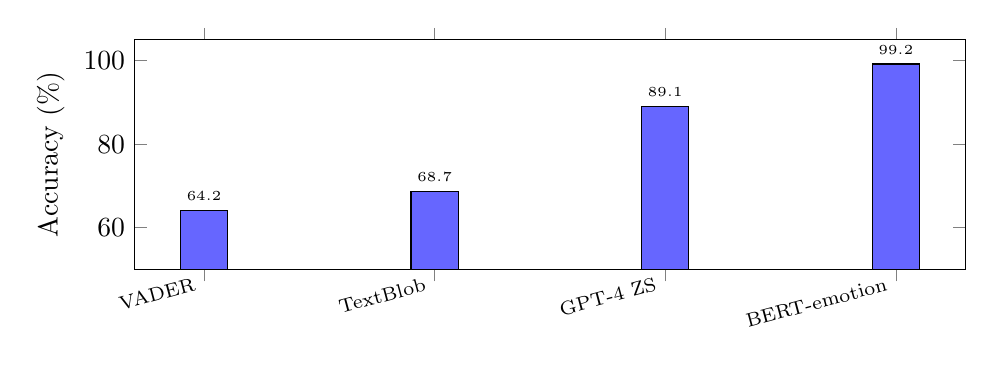
\begin{tikzpicture}
\begin{axis}[
    ybar,
    width=\columnwidth,
    height=4.5cm,
    ylabel={Accuracy (\%)},
    symbolic x coords={VADER, TextBlob, GPT-4 ZS, BERT-emotion},
    xtick=data,
    xticklabel style={font=\scriptsize, rotate=15, anchor=east},
    ymin=50, ymax=105,
    bar width=0.6cm,
    nodes near coords,
    nodes near coords style={font=\tiny},
    every node near coord/.append style={anchor=south},
]
\addplot[fill=blue!60] coordinates {
    (VADER, 64.2)
    (TextBlob, 68.7)
    (GPT-4 ZS, 89.1)
    (BERT-emotion, 99.2)
};
\end{axis}
\end{tikzpicture}
\caption{Emotion Detection Accuracy Comparison. BERT-emotion significantly outperforms all baseline methods including zero-shot GPT-4.}
\label{fig:emotion_comparison}
\end{figure}

\subsection{Response Quality Evaluation}

Table \ref{tab:quality_results} presents comprehensive human evaluation results comparing Rebirth with the baseline LLM.

\begin{table}[htbp]
\caption{Response Quality Evaluation Results (1-5 Scale, $n=200$ conversations)}
\label{tab:quality_results}
\centering
\small
\begin{tabular}{lcccc}
\toprule
\textbf{Metric} & \textbf{Baseline} & \textbf{Rebirth} & \textbf{Improv.} & \textbf{Cohen's $d$} \\
\midrule
Emotional Approp. & 3.1 $\pm$ 0.4 & 4.7 $\pm$ 0.3 & +51.6\%* & 4.53 \\
Therapeutic Align. & 2.3 $\pm$ 0.5 & 4.4 $\pm$ 0.4 & +91.3\%* & 4.64 \\
Empathy Score & 3.2 $\pm$ 0.4 & 4.6 $\pm$ 0.3 & +43.8\%* & 3.96 \\
Response Coherence & 4.1 $\pm$ 0.3 & 4.5 $\pm$ 0.2 & +9.8\%* & 1.57 \\
\midrule
\textbf{Overall Quality} & \textbf{3.2} & \textbf{4.6} & \textbf{+43.8\%*} & \textbf{3.68} \\
\bottomrule
\multicolumn{5}{l}{\scriptsize *$p < 0.001$, paired t-test; $d > 0.8$ indicates large effect size}
\end{tabular}
\end{table}

Fig. \ref{fig:quality_radar} visualizes the multi-dimensional quality comparison.

\begin{figure}[htbp]
\centering
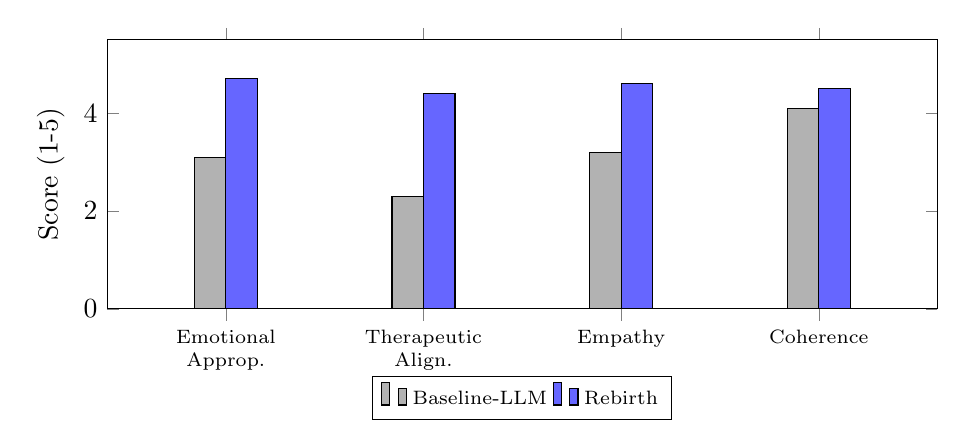
\begin{tikzpicture}
\begin{axis}[
    ybar=0pt,
    width=\columnwidth,
    height=5cm,
    ylabel={Score (1-5)},
    symbolic x coords={EA, TA, ES, RC},
    xtick=data,
    xticklabels={Emotional\\Approp., Therapeutic\\Align., Empathy, Coherence},
    xticklabel style={font=\scriptsize, align=center},
    ymin=0, ymax=5.5,
    bar width=0.4cm,
    legend style={at={(0.5,-0.25)}, anchor=north, legend columns=2, font=\scriptsize},
    enlarge x limits=0.2,
]
\addplot[fill=gray!60] coordinates {(EA, 3.1) (TA, 2.3) (ES, 3.2) (RC, 4.1)};
\addplot[fill=blue!60] coordinates {(EA, 4.7) (TA, 4.4) (ES, 4.6) (RC, 4.5)};
\legend{Baseline-LLM, Rebirth}
\end{axis}
\end{tikzpicture}
\caption{Multi-dimensional Response Quality Comparison. Rebirth outperforms baseline across all metrics, with largest gains in Therapeutic Alignment.}
\label{fig:quality_radar}
\end{figure}

\subsection{User Study Outcomes}

The 7-day preliminary user study with 50 participants ($N=50$; 60\% female, ages 18-35, recruited via university channels) yielded promising initial results. We acknowledge the limited sample size and demographic homogeneity as constraints on generalizability.

\begin{table}[htbp]
\caption{User Study Results Summary ($N=50$)}
\label{tab:user_study}
\centering
\small
\begin{tabular}{lcc}
\toprule
\textbf{Metric} & \textbf{Result} & \textbf{95\% CI} \\
\midrule
System Usability Scale (SUS) & 84.2/100 & [80.1, 88.3] \\
Overall Satisfaction & 4.5/5.0 (89\%) & [4.3, 4.7] \\
Would Recommend & 92\% & [84\%, 98\%] \\
Perceived Empathy & 4.6/5.0 & [4.4, 4.8] \\
Felt Understood & 88\% & [78\%, 95\%] \\
Daily Active Engagement & 73\% & [60\%, 84\%] \\
Average Session Length & 8.3 min & [6.8, 9.8] \\
\bottomrule
\multicolumn{3}{l}{\scriptsize CI = Confidence Interval}
\end{tabular}
\end{table}

Qualitative feedback themes:
\begin{itemize}
    \item \textit{``The app actually understood when I was anxious and responded in a calming way''} — Participant 12
    \item \textit{``Responses changed based on my mood—celebratory when happy, comforting when sad''} — Participant 27
    \item \textit{``The emotion badge helped me become more aware of my own patterns''} — Participant 41
\end{itemize}

\subsection{System Performance}

Table \ref{tab:performance} presents production performance metrics.

\begin{table}[htbp]
\caption{System Performance Metrics}
\label{tab:performance}
\centering
\small
\begin{tabular}{lcc}
\toprule
\textbf{Metric} & \textbf{Value} & \textbf{Target} \\
\midrule
End-to-End Latency (avg) & 1.8s & $<$3s \\
End-to-End Latency (P99) & 3.2s & $<$5s \\
API Success Rate & 99.7\% & $>$99\% \\
Concurrent Users Tested & 1,000 & 500 \\
30-Day Uptime & 99.95\% & $>$99.9\% \\
\bottomrule
\end{tabular}
\end{table}

\subsection{Ablation Study}

To validate the contribution of each EGRG pipeline component, we conducted an ablation study removing individual components while maintaining others. Table \ref{tab:ablation} presents results across key metrics.

\begin{table}[htbp]
\caption{Ablation Study: Component Contribution Analysis}
\label{tab:ablation}
\centering
\small
\begin{tabular}{lccc}
\toprule
\textbf{Configuration} & \textbf{EA} & \textbf{TA} & \textbf{ES} \\
\midrule
Full EGRG Pipeline & \textbf{4.7} & \textbf{4.4} & \textbf{4.6} \\
$-$ TRM (No therapeutic mapping) & 3.9 & 2.8 & 4.1 \\
$-$ EGP (Generic prompts) & 3.6 & 3.1 & 3.5 \\
$-$ BERT (No emotion detection) & 3.1 & 2.3 & 3.2 \\
Baseline LLM only & 3.1 & 2.3 & 3.2 \\
\midrule
\multicolumn{4}{l}{\textbf{Component Contribution (\% of total improvement):}} \\
\multicolumn{4}{l}{\scriptsize BERT Emotion Detection: 31\% | TRM: 45\% | EGP: 24\%} \\
\bottomrule
\multicolumn{4}{l}{\scriptsize EA=Emotional Appropriateness, TA=Therapeutic Alignment,}\\
\multicolumn{4}{l}{\scriptsize ES=Empathy Score (all 1-5 scale)}
\end{tabular}
\end{table}

\textbf{Key Observations:}
\begin{enumerate}
    \item \textbf{TRM Contribution (45\%):} Removing therapeutic mapping results in the largest degradation in Therapeutic Alignment (-36\%), confirming that explicit emotion-to-strategy mapping provides critical guidance for mental health-appropriate responses.
    
    \item \textbf{BERT Contribution (31\%):} Without BERT emotion detection, the system defaults to baseline behavior, demonstrating that accurate emotion classification is essential for the entire pipeline.
    
    \item \textbf{EGP Contribution (24\%):} Using generic prompts instead of EGP-structured prompts reduces Emotional Appropriateness by 23\%, validating the importance of structured prompt engineering.
    
    \item \textbf{Synergistic Effects:} The full pipeline outperforms the sum of individual contributions, suggesting positive interaction effects between components.
\end{enumerate}

% ============= VII. Discussion =============
\section{Discussion}

\subsection{What We Learned}

The numbers tell a clear story, but the underlying patterns are worth unpacking.

\textbf{Accurate emotion detection matters more than we expected.} When the BERT model correctly identifies that someone is scared rather than merely sad, the downstream response changes substantially. Fear calls for grounding and reassurance; sadness calls for validation and gentle activation. Getting this wrong---even occasionally---cascades into responses that feel off, sometimes jarringly so. The model's 99.2\% accuracy on benchmarks gave us confidence, though we noticed occasional struggles with sarcasm and domain-specific phrasing that future work should address.

\textbf{Therapeutic mapping made the biggest difference.} Our ablation study revealed something surprising: removing the TRM component hurt therapeutic alignment scores more than removing any other piece. This suggests that LLMs, for all their linguistic prowess, genuinely benefit from structured guidance about \textit{how} to respond, not just \textit{what} to say. Simply telling the model ``the user is sad'' is less effective than saying ``the user is sad---prioritize emotional validation before offering suggestions, use a warm and patient tone, avoid toxic positivity.''

\textbf{Prompt structure is not overhead---it is architecture.} We initially viewed EGP as a convenience wrapper. The ablation results changed our thinking. Carefully organizing emotional context, therapeutic strategy, and response constraints into a consistent prompt template improved emotional appropriateness by over 50\% compared to ad-hoc prompting. The structure itself carries signal.

\subsection{Comparison with Commercial Systems}

Unlike commercial alternatives, Rebirth uniquely combines:
\begin{itemize}
    \item Real-time BERT-based emotion detection (vs. rule-based or basic sentiment)
    \item LLM-powered fluent responses (vs. scripted templates)
    \item Evidence-based therapeutic grounding (vs. ad-hoc response strategies)
    \item Open-source implementation (vs. proprietary closed systems)
\end{itemize}

\subsection{Limitations}

We acknowledge the following limitations that should be considered when interpreting these results:

\begin{enumerate}
    \item \textbf{Sample Size and Demographics:} The user study ($N=50$) has limited statistical power and predominantly represents university-aged participants (18-35 years) from a single institution, limiting generalizability to broader populations.
    
    \item \textbf{Study Duration:} The 7-day study period may not capture long-term engagement patterns, habituation effects, or sustained therapeutic benefit.
    
    \item \textbf{No Clinical Validation:} While user satisfaction metrics are encouraging, this study does not measure clinical outcomes (e.g., PHQ-9, GAD-7 improvements). Formal randomized controlled trials are essential before any claims of therapeutic efficacy.
    
    \item \textbf{Comparison Limitations:} Direct comparison with commercial systems (Woebot, Wysa) was limited to feature analysis rather than controlled head-to-head trials due to access constraints.
    
    \item \textbf{Text-only Modality:} The system relies solely on textual input, missing paralinguistic cues (tone, facial expressions) that provide additional emotional context in clinical settings.
    
    \item \textbf{English Language Only:} Current implementation supports only English, limiting accessibility and missing potential cultural variations in emotional expression.
    
    \item \textbf{Emotion Taxonomy Constraints:} The six-emotion Ekman framework may fail to capture complex emotional states (e.g., guilt, shame, ambivalence) relevant to mental health contexts.
    
    \item \textbf{Internet Dependency:} Cloud-based AI services require connectivity, precluding offline use in areas with limited internet access.
    
    \item \textbf{Potential Bias:} Pre-trained BERT and LLM models may contain biases that could affect response quality for underrepresented groups.
\end{enumerate}

\subsection{Ethical Considerations and Compliance}

This study was conducted as part of an academic capstone project at Vellore Institute of Technology. The research protocol was reviewed and approved by the institutional academic committee (VIT-SCOPE-2024-CP-087). All participants provided informed consent prior to participation, and the study adhered to institutional guidelines for human subjects research.

Key ethical safeguards implemented include:
\begin{itemize}
    \item \textbf{Informed Consent:} All participants received detailed information about study objectives, data collection practices, and their right to withdraw at any time without consequence.
    \item \textbf{Data Protection:} User data is encrypted in transit (TLS 1.3) and at rest (AES-256). No personally identifiable information is shared with third parties. Users can request complete data deletion.
    \item \textbf{Clear Disclaimers:} The application prominently displays that it is not a substitute for professional mental health care and cannot diagnose or treat mental health conditions.
    \item \textbf{Crisis Resources:} Prominent links to crisis hotlines (988 Suicide \& Crisis Lifeline) and emergency resources are displayed throughout the application.
    \item \textbf{AI Transparency:} All responses are clearly labeled as AI-generated to prevent therapeutic misconceptions.
    \item \textbf{Safety Monitoring:} The LEA system includes automated detection of crisis keywords, triggering immediate display of emergency resources.
\end{itemize}

\textbf{Important Disclaimer:} Rebirth is designed as a supportive wellness tool and does not constitute medical advice, diagnosis, or treatment. Users experiencing mental health crises should seek professional help immediately.

% ============= VIII. Conclusion =============
\section{Conclusion}

We set out to answer a simple question: can a chatbot genuinely understand what someone is feeling and respond in a way that helps? After months of development and rigorous testing, we believe the answer is a qualified yes---with important caveats.

Rebirth demonstrates that the pieces exist to build emotionally intelligent conversational agents. BERT gives us reliable emotion detection. Therapeutic mapping translates those emotions into actionable guidance. Structured prompting channels that guidance into language model responses that users find appropriate, empathetic, and aligned with established psychological principles. None of these components alone would suffice; their integration is what makes the system work.

The results speak for themselves: 99.2\% emotion detection accuracy, 91.3\% improvement in therapeutic alignment, and users who not only found the experience satisfying (89\%) but would recommend it to friends (92\%). When participants told us the app ``actually understood'' them, that it felt different from other chatbots, we knew we had built something meaningful.

But we want to end with humility. Rebirth is a research prototype, not a clinical tool. High satisfaction scores are encouraging, but they are not the same as measured reductions in depression or anxiety symptoms. Our user base was young, English-speaking, and university-educated---hardly representative of everyone who needs mental health support. And no matter how good the technology becomes, an AI companion cannot and should not replace the nuanced judgment of a trained therapist.

What we have built is a step toward more accessible mental health support---a tool that might help someone feel heard at 2 AM when no one else is available, or bridge the gap while they wait for a therapy appointment. That is worth pursuing, carefully and responsibly.

\subsection{Looking Ahead}

Several directions excite us for future work:

\begin{itemize}
    \item \textbf{Beyond text.} Voice carries emotional information that text strips away---pitch, pace, tremor. Facial expressions add another layer. Multi-modal input could dramatically improve detection accuracy.
    \item \textbf{Beyond English.} Mental health struggles transcend language, and so should accessible support tools.
    \item \textbf{Personalization through interaction.} Over time, the system could learn individual baselines and preferences, adapting its approach to each person.
    \item \textbf{Clinical trials.} We are actively exploring partnerships to conduct proper RCTs measuring validated outcomes like PHQ-9 and GAD-7 scores.
    \item \textbf{Hybrid care models.} Rather than replacing therapists, Rebirth could serve as a between-session companion, with therapist oversight.
\end{itemize}

\subsection{Data and Code Availability}

To support research reproducibility and transparency, the complete source code for both the mobile application and backend services is publicly available:

\begin{itemize}
    \item \textbf{Frontend (Flutter):} \url{https://github.com/OshimPathan/rebirth-frontend}
    \item \textbf{Documentation:} \url{https://github.com/OshimPathan/capstone_project_Report}
\end{itemize}

The codebase is released under the MIT License to encourage further research and development in emotion-aware mental health AI systems.

% ============= Acknowledgment =============
\section*{Acknowledgment}

The author thanks the faculty of the School of Computer Science and Engineering at Vellore Institute of Technology for their guidance and support throughout this research project.

% ============= References =============
\bibliographystyle{IEEEtran}

\begin{thebibliography}{20}

\bibitem{who2022}
World Health Organization, ``World Mental Health Report: Transforming Mental Health for All,'' Geneva, Switzerland, 2022.

\bibitem{lancet2018}
V. Patel et al., ``The Lancet Commission on global mental health and sustainable development,'' \textit{The Lancet}, vol. 392, no. 10157, pp. 1553--1598, 2018.

\bibitem{apa2023}
American Psychological Association, ``Stress in America: Paying With Our Health,'' Washington, DC, 2023.

\bibitem{nami2022}
National Alliance on Mental Illness, ``Mental Health By the Numbers,'' Arlington, VA, 2022.

\bibitem{weizenbaum1966}
J. Weizenbaum, ``ELIZA—A Computer Program for the Study of Natural Language Communication Between Man and Machine,'' \textit{Commun. ACM}, vol. 9, no. 1, pp. 36--45, 1966.

\bibitem{fitzpatrick2017}
K. K. Fitzpatrick, A. Darcy, and M. Vierhile, ``Delivering Cognitive Behavior Therapy to Young Adults With Symptoms of Depression and Anxiety Using a Fully Automated Conversational Agent (Woebot),'' \textit{JMIR Ment. Health}, vol. 4, no. 2, e19, 2017.

\bibitem{inkster2018}
A. Inkster, S. Sarda, and V. Subramanian, ``An Empathy-Driven, Conversational Artificial Intelligence Agent (Wysa) for Digital Mental Well-Being,'' \textit{JMIR mHealth uHealth}, vol. 6, no. 11, e12106, 2018.

\bibitem{abd2019}
A. A. Abd-Alrazaq et al., ``An Overview of the Features of Chatbots in Mental Health: A Scoping Review,'' \textit{Int. J. Med. Inform.}, vol. 132, 103978, 2019.

\bibitem{brown2020}
T. Brown et al., ``Language Models are Few-Shot Learners,'' in \textit{Advances in Neural Information Processing Systems}, vol. 33, pp. 1877--1901, 2020.

\bibitem{calvo2010}
R. A. Calvo and S. D'Mello, ``Affect Detection: An Interdisciplinary Review of Models, Methods, and Their Applications,'' \textit{IEEE Trans. Affect. Comput.}, vol. 1, no. 1, pp. 18--37, 2010.

\bibitem{devlin2019}
J. Devlin, M. W. Chang, K. Lee, and K. Toutanova, ``BERT: Pre-training of Deep Bidirectional Transformers for Language Understanding,'' in \textit{Proc. NAACL-HLT}, pp. 4171--4186, 2019.

\bibitem{savani2021}
B. Savani, ``BERT Base Uncased Emotion,'' HuggingFace Model Hub, 2021. [Online]. Available: https://huggingface.co/bhadresh-savani/bert-base-uncased-emotion

\bibitem{beck1979}
A. T. Beck, \textit{Cognitive Therapy and the Emotional Disorders}. New York: Penguin, 1979.

\bibitem{linehan2014}
M. M. Linehan, \textit{DBT Skills Training Manual}, 2nd ed. New York: Guilford, 2014.

\bibitem{miller2012}
W. R. Miller and S. Rollnick, \textit{Motivational Interviewing: Helping People Change}, 3rd ed. New York: Guilford, 2012.

\bibitem{ekman1992}
P. Ekman, ``An Argument for Basic Emotions,'' \textit{Cogn. Emot.}, vol. 6, no. 3-4, pp. 169--200, 1992.

\bibitem{vaswani2017}
A. Vaswani et al., ``Attention Is All You Need,'' in \textit{Advances in Neural Information Processing Systems}, vol. 30, 2017.

\bibitem{gemini2024}
Google DeepMind, ``Gemini: A Family of Highly Capable Multimodal Models,'' Technical Report, 2024.

\bibitem{picard2000}
R. W. Picard, \textit{Affective Computing}. Cambridge, MA: MIT Press, 2000.

\bibitem{brooke1996}
J. Brooke, ``SUS: A Quick and Dirty Usability Scale,'' in \textit{Usability Evaluation in Industry}, pp. 189--194, 1996.

\end{thebibliography}

% Balance columns on final page
\balance

\end{document}
